\documentclass[russian]{lecture-notes}

\usepackage{dsfont}
\usepackage[final]{graphicx}
\usepackage[normalem]{ulem}
\usepackage{amsmath}
\usepackage{amsfonts}
\usepackage{amssymb}
\usepackage{tikz}
\usepackage{svg}
\usepackage{timestamps}
\usepackage{algorithm}
\usepackage{algpseudocode}

\title{Бесконечные цепные дроби. Простые числа. Основная теорема арифметики.}
\lecturer{Поздняков Сергей Николаевич}
\notesauthor{Ковалева Ксения}
\date{12.03.2018}

\begin{document}
	\youtubevideo{NBAODXj3NFY}
	
	\maketitle
	\section*{Бесконечные цепные дроби}
	\timestamp{10:10}
	
	Рассмотрим в качестве примера выражение, которое, может определять число или быть какой-то иной конструкцией. С этим нам и придется разобраться.
	\begin{example*}
		$$1+\frac{1}{2+\frac{1}{1+\frac{1}{1+\frac{1}{2+\frac{1}{1+\frac{1}{1+\frac{1}{2+...}}}}}}}$$
		
		Здесь можно увидеть некоторую закономерность (дробь написана так, чтобы был виден период). Может показаться, что период начинается с первой двойки, но на самом деле можно заметить, что период начинается несколько позже: (1,1,2).
		
		Всю эту дробь можно представить в виде начала и периода, то есть: $[1;2,(1,1,2)]$. Это пример \textit{периодической цепной дроби}.
		
		Предположим, что в данной записи есть смысл (чуть позже мы его определим через предел: если бы мы сначала вычислили первую подходящую дробь, затем вторую, тетью и т.д. и выяснилось бы, что последовательность подходящих дробей имеет предел, то его и следовало бы считать значением этого выражения (допустим, $\alpha$)).
		
		Воспользуемся этим предположением, т.е. тем, что он существует. Выделим периодическую часть отдельно ($x$) от общего выражения ($\alpha$) и рассмотрим, чему бы она тогда была равна, если мы можем утверждать, что такой предел существует:
		
		$$1+\frac{1}{1+\frac{1}{2+\frac{1}{1+\frac{1}{1+\frac{1}{2+\frac{1}{1+...}}}}}}$$
		
		Посмотрим на эту дробь следующим образом: выделим нижнюю часть выражения.$$1+\frac{1}{1+\frac{1}{2+\frac{1}{1+...}}}$$ 
		Чем этот кусочек отличается от всей дроби? Видно, что ничем, потому что она бесконечная, и не важно, с какого периода начать, она все равно будет одинакова. (Подобная структура встречается во фракталах: сдвинули -- получили то же самое).
		
		Тогда мы можем свести выражение к такому уравнению: $$x = 1+\frac{1}{1+\frac{1}{2+\frac{1}{x}}}$$
		
		Какой степени буудет это уравнение (квадратное, кубическое и т.д.) сразу не догадаться, поэтому предлагается использовать быстрый способ вычисления правой части. Её можно рассмотреть как конечную цепную дробь, у которой первый член - единица, второй - единица, третий - двойка, а последний - $x$. Изобразим уже знакомую нам таблицу и вычислим подходящие дроби:
		
		\begin{center}
			\begin{tabular}{|c|c|c|c|c|c|}
				\hline
				& & 1 & 1 & 2 & $x$\\\hline
				0 & 1 & 1 & 2 & 5 & $2+5\cdot x$\\\hline
				1 & 0 & 1 & 1 & 3 & $1+3\cdot x$ \\\hline
			\end{tabular}
		\end{center}
		
		Тогда получается такое уравнение: $\frac{2+5\cdot x}{1+3\cdot x}=x$. Чтобы увидеть его канонический вид, остается один шаг. Умножаем уравнение на знаменатель и получаем $3x^2-4x-2=0$. Обратите внимание, почему мы стали вычислять эту дробь именно через подходящие? Потому что теперь достаточно легко доказать, что каким бы ни был период,  уравнение будет квадратным, потому что до последнего столбца в таблице все элементы не будут содержать $x$, а появится он только на последнем шаге. Поэтому уравнение всегда будет иметь вид $\frac{a+b\cdot x}{c+d\cdot x}=x$ и всегда будет квадратным.
		
		Дальше действуем как обычно, решаем уравнение и получаем корни:
		\begin{center}
			$x_{1,2}=\frac{2\pm \sqrt{4+6}}{3}$
		\end{center} 
	
		Отрицательный корень можно сразу отбросить, потому что все элементы дроби положительные и отрицательной она быть не может, получается:
		\begin{center}
			$x=\frac{2+\sqrt{10}}{3}$
		\end{center} 
		
		Дальше мы можем вычислить $\alpha$, подставив вместо $x$ это выражение: \begin{center}
			$\alpha=1+\frac{1}{2+\frac{3}{2+\sqrt{10}}}$
		\end{center} 
		
		\begin{remark}
			Понятно, что такое выражение можно считать <<снизу вверх>>, но, опять же, лучше считать его <<сверху вниз>> (слева направо при линейной записи). Особенно это удобно, если дробь длинная: сначала находим подходящую дробь, а вместо всего остального оставляем $x$, и на последнем шаге получается уже знакомое выражение вида $\frac{a+b\cdot x}{c+d\cdot x}=x$. Дальше мы находим корень, домножаем на сопряженное и всегда получаем выражение вида $\frac{a+b\sqrt{D}}{c}$, где $a, b, c \in \mathbb{Z}$. Если мы хотим, чтобы $b$ в выражении не было, его можно внести под корень.
		\end{remark}
	\end{example*}

	Можно предположить, что не только периодические, но и произвольные цепные бесконечные дроби имеют смысл, т.е. могут представлять какие-то числа. Но для этого надо доказать, что у последовательности их подходящих дробей всегда будет предел, который и будем считать значением цепной дроби.

	\begin{theorem}
		Последовательность подходящих дробей всегда имеет предел.
	\end{theorem}
	\begin{proof}
		Пусть: $\alpha = q_1+\frac{1}{q_1+...\frac{1}{q_n+...}}$ - бесконечная цепная дробь\newline $\frac{P_0}{Q_0};\frac{P_1}{Q_1};...;\frac{P_n}{Q_n}$ - последовательность подходящих дробей\vspace{1mm}\newline
		Тогда существует предел $\alpha=\lim_{n\to \infty} \frac{P_n}{Q_n}$, который мы будем считать значением цепной дроби.\vspace{3mm}\newline
	\end{proof}
	
	Для того, чтобы доказать предел, надо вспомнить, какие есть теоремы о пределах. Для этого нам надо знать свойства последовательностей подходящих дробей.
	
	\timestamp{21:51}
	\section*{Свойства подходящих дробей:}
	\begin{enumerate}
		\item {$\frac{P_n}{Q_n}$ - несократима}
		
		\item {Если мы возьмем разность соседних дробей, то получится $\frac{P_n}{Q_n}-\frac{P_{n-1}}{Q_{n-1}}=\frac{P_n\cdot Q_{n-1}-P_{n-1}\cdot Q_n}{Q_n\cdot Q_{n-1}}=\frac{(-1)^{n-1}}{Q_n\cdot Q_{n-1}}$}
		
		\item {Если взять подпоследовательность четных дробей $\frac{P_{2n}}{Q_{2n}}$, то она возрастает, а последовательность нечетных $\frac{P_{2n-1}}{Q_{2n-1}}$ будет убывать}
		
		\item {Если $\alpha$ - число, заданное цепной дробью, то все четные лежат левее его, а все нечетные, наоборот, правее:
			
		$\frac{P_{2n}}{Q_{2n}}\leq \alpha $
		
		$\frac{P_{2n-1}}{Q_{2n-1}} \geq \alpha$}
	\end{enumerate}

	Докажем некоторые из свойств:
	\begin{enumerate}
		
		\item \begin{proof}
		\timestamp{26:24}

		В прошлой лекции была сформулирована идея об использовании сходстве расширенного алгоритма Евклида с алгоритмом генерации подходящих дробей для доказательства свойств послнедних. Применим её для доказательства базовых свойств, а остальные выведем из них.
		
		Итак, у нас есть некоторая бесконечная цепная дробь:
		
		$\alpha=q_1+\frac{1}{q_1+...\frac{1}{q_n+...}}$
		
		Рассмотрим подходящие дроби $\frac{P_n}{Q_n}$ и <<оборвём>> последовательность на $ n$-ом шаге. Это означает, что из цепной дроби удалили все члены после $ n$-ого. Получится конечная цепная дробь $[q_0;q_1,...,q_n]$. Ей будет соответствовать обыкновенная дробь $a$/ $b$, которая равна последней подходящей дроби $\frac{P_n}{Q_n}$.
		
		Рассмотрим алгоритм Евкдида: обычный и расширенный. В качестве $a$ будет $P_n$, в качестве $b$ - $Q_n$.
		
		\begin{center}
			\begin{tabular}{|c|c|c|c|c|c|}
				\hline
				$a=P_n$ & $b=Q_n$ & $r_0$ &  & $d$ & $r_n=0$ \\\hline
				&  & $q_0$ & ... & ... & $q_n$ \\\hline
				1 & 0 & $x_0$ &  & $x_{n-1}$ & $x_n$ \\\hline
				0 & 1 & $y_0$ &  & $y_{n-1}$ & $y_n$ \\\hline
			\end{tabular}
		\end{center}
		
		Поскольку на $ n$-ом шаге алгоритм должен завершиться (раз $q_n$ - последняя), значит $r_n$ должен равняться нулю, а в предыдушем столбце должен быть наибольший общий делитель $d =$ НОД$(a, b)$ -- по смыслу алгоритма Евклида. В этом столбце также содержатся коэффициенты линейного представления НОД: $x_{n-1}$ и $y_{n-1}$.
		\end{proof}
	
		Ранее мы доказали теорему о том, что 
		\begin{equation}
			x_{n-1}a + y_{n-1}b = d
		\end{equation}
		
		Если $x_{n-1}$ и $y_{n-1}$ не взаимно простые, то НОД$(x_{n-1}, y_{n-1}) = d' > 1$. Тогда $x_{n-1} \vdots d', a \vdots d, y_{n-1} \vdots d', b \vdots d$. Мы получаем, что если все сократить на $d$, в правой части будет единица, которая должна еще делиться на $d'$, поэтому из этого равенства следует, что $d'$ может быть равно только единице. Из (1) следует, что $d' = 1$. Противоречие. (Если доказывать не от противного, то мы просто найдем, что наибольший общий делитель равен единице).
		
		Мы доказали, что коэффициенты $x_{n-1}$ и $y_{n-1}$ взаимно простые.
		
		\begin{remark}
			На прошлой лекции было доказано, что $x$ и $y$ связаны очень простыми формулами с $P_n$ и $Q_n$: \\
			$x_n = (-1)^nQ_n$\\
			$y_n = (-1)^{n-1}P_n$,\\
			поэтому $P_n$ и $Q_n$ тоже взаимно простые. 
		\end{remark}
	
		\item \begin{proof}
		\timestamp{32:45}
		
			Итак, получается, что все подходящие дроби несократимы. Теперь выясним, почему числитель выражения\\ $\frac{P_n\cdot Q_{n-1}-P_{n-1}\cdot Q_n}{Q_n\cdot Q_{n-1}}$ обязательно равен $1$ или $-1$. Для этого используем доказанное выше  и подставим в выражение
		\begin{equation}
			x_{n-1}a + y_{n-1}b = d
		\end{equation}
			 $x_{n-1} = (-1)^{n-1}Q_{n-1}$, $y_{n-1} = (-1)^nP_{n-1}$, $a=P_n$, $b=Q_n$, $d = 1$.\\
			Получим $(-1)^{n-1}Q_{n-1}P_n + (-1)^nP_{n-1}Q_n = 1$ \\
			Домножим на $(-1)^{n-1}$ и получим $P_n\cdot Q_{n-1}-P_{n-1}\cdot Q_n = (-1)^{n-1}$.
		\end{proof}
		
		\item \begin{proof}
			\timestamp{36:22}
			Итак, мы доказали формулу о разности соседних подходящих дробей, и теперь выведем из неё следствия. Как ведут себя знаменатели дроби $\frac{(-1)^{n-1}}{Q_n\cdot Q_{n-1}}$ при росте $n$? Используем полученную на предыдущей лекции рекуррентную формулу\\ $Q_{n+1} = Q_{n-1} + a_{n+1}Q_n$. Понятно, что в какой-то момент $Q_{n-1}$ становится больше нуля, как и следующие два члена равенства, но это натуральные числа, значит на каждом шаге $Q_n$  будет увеличиваться по крайней мере на единичку, поэтому дробь $\frac{(-1)^{n-1}}{Q_n\cdot Q_{n-1}}$ при росте $Q_n$ будет стремиться к нулю, а разница между соседними подходящими дробями будет уменьшаться и стремиться к нулю. 
					
			Теперь по аналогии с проделанными выкладками, рассмотрите самостоятельно разности ближайших дробей с четными номерами и отдельно с нечетными. У вас должно получиться, что последовательность с чётными номерами возрастает, а с нечтеными -- убывает. Итак, мы имеем две последовательнности: одна из них монотонно возрастает (это четная), вторая монотонно убывает (нечетная). Изобразим свойства подходящих дробей такой картинкой:
			
			\centering
			\tikz{
				\draw (0,0) -- (4,0) arc (0:180:2) (4,0) arc (0:180:1.5) (1,0) arc (180:0:1) (3,0) arc (0:180:0.5);
				
				\coordinate [label=below:$\frac{P_0}{Q_0}$] (A) at (0,-0.25);
				\coordinate [label=below:$\frac{P_1}{Q_1}$] (B) at (4,-0.25);
				\coordinate [label=below:$\frac{P_2}{Q_2}$] (C) at (1,-0.25);
				\coordinate [label=below:$\frac{P_3}{Q_3}$] (D) at (3,-0.25);
				
				\draw [<-] (4,0) arc (0:90:2);
				\draw [<-] (1,0) arc (180:90:1.5);
				\draw [<-] (3,0) arc (0:90:1);
				\draw [<-] (2,0) arc (180:90:0.5);
			}
			\flushleft
			Получается, что есть две последовательности, члены одной лежат левее другой, левая последовательность возрастает, а правая убывает. По теореме Вейрштрасса об ограниченной монотонной последовательности у обеих последовательностей будут пределы.  В то же время расстояние между последовательносями стремится к нулю, значит предел у обеих последовательностей один и тот же. Обозначим его $\alpha$ и назовем значением бесконечной цепной дроби. \\
			Вернемся к периодической цепной дроби: мы уже поняли на примере, что если брать периодическую дробь, то будет получаться квадратичная иррациональность, и это мы доказали. Остается вопрос: любая ли квадратичная иррациональность представляется периодической цепной дробью? Это более трудная задача, и желающие могут попробовать её решить самостоятельно или найти ответ в литературе (например, в книге А.Я.Хинчина <<Цепные дроби>>. Корень можно рассматривать в широком смысле как $\frac{a+b\sqrt{D}}{c}$, а можно рассмотреть просто корень из $n$, все равно задача будет такой же сложности.
		\end{proof}
		
	\end{enumerate}
	\newpage
	\timestamp{40:32}
	Теперь рассмотрим пример, который обобщает алгоритм Евклида и показывает, как разлагать число в непрерывную цепную дробь.
	
	\section*{Алгоритм разложения числа в цепную дробь}
	
	Для начала рассмотрим простой пример, а затем напишем этот алгоритм уже формально.
	
	\begin{example*}
		$\sqrt{3}$
	
		Когда число было обычной дробью, мы делили числитель на знаменатель, выделяли целую часть и далее повторяли это процесс для дроби из делителя и остатка. Но целую часть мы можем выделить из любого числа, не обязательно применяя алгоритм Евклида, а используя какой-либо другой алгоритм. 
		
		\begin{remark}
			Обратите внимание, что хотя в заголовке написано \textit{алгоритм}, на самом деле это несколько рискованно, потому что выделение целой части разных чисел (или их классов) может потребовать разных приемов (алгоритмов), и не очевидно сразу, что такие алгоритмы есть. Поэтому преподаватель не утверждает, что знает все такие алгоритмы и как, скажем, число $\pi$ разлагать в цепную дробь, и  какой для этого понадобится алгоритм нахождения целой части сразу сказать нельзя.
			
			Но, например, для квадратичных иррациональностей вы сможете догадаться сами, как запрограммировать алгоритм, который мы разберем на примере и вы освоите его при выполнении индивидуального домашнего задания (может быть, кто-нибудь это реализует его как приложение в системе компьютерной алгебры, которая будет создаваться в рамках коллоквиума).
		\end{remark}
	
		Имеем $\sqrt{3} = 1 + (\sqrt{3} - 1)$
		
		Первое слагаемое -- целая часть, а вторая -- дробная. Теперь дробную часть можно записать в таком виде:
		
		$\sqrt{3} = 1 + (\sqrt{3} - 1) = 1 + \frac{1}{\frac{1}{\sqrt{3}-1}}$
		
		C тем, что стоит в знаменателе второго слагаемого, можно сделать такое преобразование как домножение на сопряженное (на $\sqrt{3} + 1$). Получится:
		
		$\sqrt{3} = 1 + (\sqrt{3} - 1) = 1 + \frac{1}{\frac{1}{\sqrt{3}-1}} = 1 + \frac{1}{\frac{\sqrt{3}+1}{2}}$ (т.к. мы получили в знаменателе разность квадратов $3 - 1 = 2$)
		
		Мы привели равенство к такому виду, которое позволяет нам дальше действовать рекурсивно: мы опять получили в знаменателе некоторое число, которое всегда больше единицы (почему оно всегда больше единицы? Потому что дробная часть всегда меньше, поэтому единица, деленная на это число, всегда больше), и этот процесс можно повторить.
		
		$\sqrt{3} = 1 + (\sqrt{3} - 1) = 1 + \frac{1}{\frac{1}{\sqrt{3}-1}} = 1 + \frac{1}{\frac{\sqrt{3}+1}{2}} = 1 + \frac{1}{1+\frac{\sqrt{3}-1}{2}}$\\ (Так как 1< $\sqrt{3}$ < 2, целая часть корня равна 1, тогда целая часть <<числителя знаменателя>> равна 2, а целая часть всего знаменателя 1).
		
		Есть такая опасность, что кто-то, увидев в целой части единицу, и в знаменателе дробной части единицу, решит, что на этом работа закончена и получилась периодическая дробь с периодом из единиц. На самом деле, это преждевременное утверждение: мы не можем утверждать, что период есть, пока дробная часть не повторится. В нашем случае дробные части разные, поэтому надо работать дальше. 
		
		Повторяя операции <<переворачивания>>, домножения на сопряженное и выделения целой части, получаем:
		
		$\sqrt{3} = 1 + \frac{1}{1+\frac{\sqrt{3}-1}{2}} = 1 + \frac{1}{1+\frac{2}{\sqrt{3}-1}} = 1 + \frac{1}{1+\frac{1}{\sqrt{3}+1}} = 1 + \frac{1}{1+\frac{1}{2 + (\sqrt{3}-1)}}$ 
		
		И вот теперь обратим внимание, что мы получили ту же самую дробную часть, что и была изначально, а значит, дальше процессс начнет повторяться: снова появится единица и так далее. Получаем период $(1,2)$. Так как зацикливание не затронуло первый член дроби, записать результат можно как $[1; (1,2)]$
	\end{example*}

	\timestamp{1:04:44}
	И, наконец, сформулируем алгоритм разложения числа в цепную дробь (который ссылается на неизвестный в общем виде алгоритм выделения целой части).
	Поскольку бесконечно  работать алгоритм не может,   мы будем задавать число шагов $n$ и останавливать алгоритм <<искусственно>>.
	
	\begin{algorithm}[H]
		\caption{Алгоритм разложения числа в цепную дробь}
		\label{alg:klass}
		\begin{algorithmic}[1]
			\State $x := \alpha$;
			\Comment $\alpha$ -- исходное число.
			\State $i := 0$;
			\Comment $i$ -- номер члена цепной дроби.
			\While {$x \neq 0$ и $i \leq n$}
			\State $q[i] := int(x)$;
			\Comment $q[i]$ -- целая часть $x$.
			\State $x := \frac{1}{x-q[i]}$;
			\State $i := i + 1$;
			\EndWhile
		\end{algorithmic}
	\end{algorithm}
			
	То есть, мы все время выполняем две операции: берем целую часть, потом единицу делим на дробную часть и снова выделяем из неё целую часть.
	
	Теперь давайте разберем главное назначение цепных дробей. Выполнять арифметические операции над цепными дробями не просто трудно, а скорее невозможно, то есть сложить их, умножить -- нереально. А вот что полезного можно делать с цепными дробями -- это искать рациональные приближения вещественных чисел, поэтому сейчас мы рассмотрим теорему о наилучшем приближении. (По данным из Википедии, она уже называется диофантовым приближением, хотя раньше так никто не говорил)
	
	\begin{definition} 
	\timestamp {47:50}
		Дробь $\frac{a}{b}$ называется наилучшим приближением к числу $\alpha$, если у любой дроби $\frac{x}{y}$, которая лежит ближе, знаменатель больше, то есть 
		
		$|\alpha - \frac{x}{y}| < |\alpha - \frac{a}{b}| \Rightarrow y > b$ 
		
	\end{definition}

	\begin{remark}
		Другая формулировка (отрицательная формулировка определения): не существует дроби, которая была бы ближе к $\alpha$, а знаменатель у нее был бы такой же или меньше. 
	\end{remark}	
	
	Теперь, как вы догадались, нужно доказать, что все наши подходящие дроби являются наилучшими приближениями.
		
		Для начала докажем такую лемму:
		\begin{lemma}
			Пусть $\frac{x}{y} \in (\frac{a}{b}; \frac{c}{d})$ такому, что дроби промежутка обладают свойством двух соседних подходящих дробей, то есть если вычесть из правой левую, то в числителе получится единица:
			
			$\frac{c}{d} - \frac{a}{b} = \frac{cb-ad}{db} = \frac{1}{db}$, потому что мы вычитали из большего меньшее (промежуточная выкладка)
			
			То есть условие выглядит так: $bc - ad = 1$. 
			\\При таком условии знаменатель дроби будет больше знаменателей концов промежутка: $y > b, y > d$. Иными словами,  в таких промежутках все рациональные числа <<плохие>> и в качестве наилучшего приближения надо брать один из концов промежутка.
		\end{lemma}
		\begin{proof}
			Для доказательства вычислим разность $\frac{x}{y} - \frac{a}{b}$. Оценим её сверху: 
			
			$\frac{x}{y} - \frac{a}{b} < \frac{c}{d} - \frac{a}{b} = \frac{bc-ad}{bd} = \frac{1}{bd}$ - по условию.
			
			Теперь оценим её снизу. Для начала просто посчитаем:
			
			$\frac{x}{y} - \frac{a}{b} = \frac{bx-ay}{by}$
			
			Числитель является положительным? Да, потому что $\frac{x}{y}$ лежит справа от $\frac{a}{b}$. Раз он положительный и, кроме того, целый, значит, он по крайней мере равен единице, то есть можно сказать, что $\frac{bx-ay}{by} \geq \frac{1}{by}$
			
			А теперь сравните: с одной стороны мы написали, что $\frac{x}{y} - \frac{a}{b}$ меньше $\frac{1}{bd}$, а с другой стороны написали, что $\frac{x}{y} - \frac{a}{b}$ больше $\frac{1}{by}$. Можно утверждать, что $\frac{1}{bd}$ будет больше $\frac{1}{by}$. 
			
			$\Rightarrow \frac{1}{bd} > \frac{1}{by} \Rightarrow y > d$. Половина леммы доказана.
			
			В качестве упражнения докажите второе неравенство ($y > b$) самостоятельно.
		\end{proof}	
		
	Также следует упомянуть важное следствие, ради чего мы и доказывали лемму: 
	\begin{theorem} 
		Все подходящие дроби, начиная с $\frac{P_1}{Q_1}$ (все, кроме $\frac{P_0}{Q_0}$), являются наилучшими приближениями к числу $\alpha = q_0 + \frac{1}{q_1 + ... + \frac {1}{q_n ...}}$.
	\end{theorem}
	\begin{proof}
		Рассмотрим промежуток между соседними подходящими дробями $\frac{P_{n-1}}{Q_{n-1}}$ и $\frac{P_n}{Q_n}$. Мы будем брать разность по модулю, потому что для разных значений $n$ она может иметь разный знак. По свойству 2 подходящих дробей будем иметь:
		
		$|\frac{P_{n-1}}{Q_{n-1}} - \frac{P_n}{Q_n}| = \frac{1}{Q_{n-1}Q_n}$
		
		То есть, выполнены условия леммы. 
		
		Если $\alpha$ лежит в промежутке между $\frac{P_{n-1}}{Q_{n-1}}$ и $\frac{P_n}{Q_n}$ (мы не указываем, какая дробь слева, а какая справа, потому что нам это неизвестно), то можно утверждать, что если какая-то дробь лежит ближе, чем $\frac{P_n}{Q_n}$, то
		
		$|\alpha - \frac{x}{y}| < |\alpha - \frac{P_n}{Q_n}| \Rightarrow  \frac{x}{y} \in (\frac{P_{n-1}}{Q_{n-1}}; \frac{P_n}{Q_n}) \Rightarrow  y > Q_n$ (заметим, что границы последнего промежутка могут меняться местами в зависимости от $n$).
		
		Почему первая дробь (с индексом 0)  не всегда будет подходящей? 
		
		\centering
		\tikz{
			\draw (0,0) -- (4,0) arc (0:180:2);
			\draw [fill=black] (3,0) circle (0.4 mm);
			\draw [very thick](2,0) -- (4,0);
		
			\coordinate [label=center:$($] (E) at (2,0);
			\coordinate [label=center:$)$] (F) at (3.98,0);
			\coordinate [label=below:$\frac{P_0}{Q_0}$] (A) at (0,-0.25);
			\coordinate [label=below:$\frac{P_1}{Q_1}$] (B) at (4,-0.25);
			\coordinate [label=below:$\frac{P_2}{Q_2}$] (C) at (2,-0.25);
			\coordinate [label=below:$\alpha$] (D) at (3,-0.25);
			
		}
		\flushleft
		
		Потому что из условия  $|\alpha - \frac{x}{y}| < |\alpha - \frac{P_0}{Q_0}|$  не следует, что  $\frac{x}{y} \in (\frac{P_0}{Q_0}; \frac{P_1}{Q_1})$.
		
		Мы можем подобрать такой пример, как $\frac{19}{10} = 1 + \frac{9}{10} = 1 + \frac{1}{1+\frac{1}{9}}$. 
		
		И вот, подходящие дроби: $\frac{P_0}{Q_0} = \frac{1}{1}, \frac{P_1}{Q_1} = 1 + \frac{1}{1} = \frac{2}{1}$. Понятно, что если мы возьмем первую дробь, она наилучшим приближением не будет, потому что вторая дробь -- двойка -- ближе к изначальному числу, а знаменатель её не больше единицы. \\
		Тема для исследования: оказывается не только подходящие дроби могут быть наилучшими приближениями. Есть еще так называемые \textit{промежуточные} дроби, которые тоже являются подходящими. Они, в некотором смысле, <<хуже>> обычных подходящих. Предлагается найти способ построения таких дробей.
		
	\end{proof}
		
	\section*{\S 11. Простые числа. Основная теорема арифметики.}		
	\timestamp {1:07:51}
		
	С определением простого числа вы уже знакомы: это число, которое не имеет других делителей, кроме единицы и себя. Единицу для удобства простым числом не считают, поэтому берут числа с этим свойством большие единицы. 
	
	\begin{definition}
		$p$ -- простое по определению, если $p > 1$ и не имеет других делителей, кроме 1 и $p$ ($p \in \mathbb{N}$).
	\end{definition}

	Сначала на примере попробуем самый естественный алгоритм генерации простых чисел (можно реализовать на коллоквиуме по системам компьютерной алгебры) - решето Эратосфена.
		
	\begin{example*} [Решето Эратосфена]
		
		Рассмотрим небольшой отрезок натурального ряда, для удобства поместив его в таблицу:\\
		
		\begin{center}
			\begin{tabular}{|c|c|c|c|c|c|}
				\hline
				1 & 2 & 3 & 4 & 5 & 6\\\hline
				7 & 8 & 9 & 10 & 11 & 12\\\hline
				13 & 14 & 15 & 16 & 17 & 18\\\hline
				19 & 20 & 21 & 22 & 23 & 24\\\hline 
				25 & 26 & 27 & 28 & 29 & 30\\\hline 
				31 & 32 & 33 & 34 & 35 & 36\\\hline 
				37 & 38 & 39 & 40 & 41 & 42\\\hline 
				43 & 44 & 45 & 46 & 47 & 48\\\hline
				... & ... & ... & ... & ... & ...\\\hline
			\end{tabular}
		\end{center}
		
		Алгоритм начинается с того, что, во-первых, единицу мы просто не считаем и вычеркиваем. Далее берем первое из чисел, которое не вычернуто: у нас это двойка. Это число \textit{обязательно будет простым}. Затем вычеркиваем все числа, которые на него делятся, то есть вычеркиваем каждое второе. Первое невычеркнутое число -- три -- \textit{следующее простое число}. Вычеркиваем каждое третье число. Получаем новое простое число -- пять  (первое невычеркнутое) и вычеркиваем все числа, кратные 5. Следующее простое число -- семь. Нужно ли вычеркнуть теперь каждое седьмое, чтобы получить очередное простое на нашем отрезке натурального ряда? Оказывается, нет! Все требуемые простые числа уже получены -- все невычеркнутые числа. Дальше числа если и делятся на 7, то их частными будут 2, 3 и так далее, а такие числа уже вычеркнуты, значит, следующий невычеркнутый вариант -- 49, но такого числа в нашем отрезке натурального ряда уже нет. Значит, все оставшиеся невычеркнутые числа - простые. 
		\newline
		\begin{figure}[h]
			\centering
			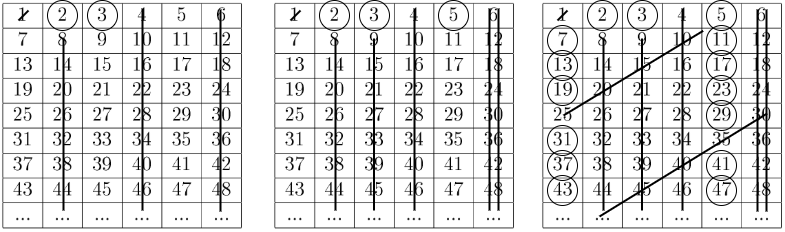
\includegraphics[width=1\textwidth]{resheto}
		\end{figure}
		
		Прелесть решета Эратосфена в том, что за $n$ проходов получаются все простые числа от 1 до $n^{2}$.
		
	\end{example*}
		
	А теперь классическая теорема о том, почему простых чисел бесконечно много. На первый взгляд, это очевидно, но если задуматься, то возникает вопрос, а почему бы, начиная с некоторого $n$, следующие за ним числа не делились на какое-нибудь из предыдущих? Сразу не скажешь, что это очевидно.
		
	\begin{theorem*}
		\timestamp{1:13:25}
		Количество простых чисел бесконечно. 
	\end{theorem*}
	\begin{proof} [Доказательство (от противного)]
		
		Пусть у нас есть конечное число простых чисел: $p_1, p_2, ..., p_n$ -- других нет.
			
		Построим новое число по такому принципу: перемножим все эти числа и добавим единицу. 
			
		$N = p_1p_2...p_n + 1$. Как вы считаете, делится ли это число на $p_1$? Нет, потому что будет остаток 1 при делении. При делении на $p_2$ также будет остаток 1, и так далее, то есть, $N$ не делится ни на одно из этих чисел, тогда оно простое по определению -- противоречие с условием.
	\end{proof}
	
	\begin{theorem*} [Основная теорема арифметики]
		\timestamp{1:15:23}
		 Любое натуральное число единственным способом (с точностью до порядка) представляется произведением простых чисел.
	\end{theorem*}
	\begin{proof}
		
		Пусть у нас есть число $N$. Есть два варианта: делится оно на что-нибудь или не делится. Если оно не делится ни на какое число, меньшее $N$, но большее единицы, то оно само простое. Второй вариант -- есть простой делитель, допустим, $p_1$. Тогда мы представляем число в виде 
		
		$N = p_1 \cdot N_1$. Дальше повторяем этот процесс с $N_1$ и т.д.
		Понятно, что этот процесс рано или поздно остановится, потому что у нас на каждом шаге с $N_i$ будет  меньше предыдущего, поэтому этот процесс остановится, и у нас получится некоторое произведение чисел, которые уже не разлагаются, то есть являются простыми. Мы их, как всегда, упорядочим по возрастанию (одинаковые сомножители запишем в виде степени):
		
		$N = p_1 \cdot N_1 = ... = {p_1}^{k_1} {p_2}^{k_2} ... {p_n}^{k_n}$
		
		Почему это произведение единственное? Почему нельзя разложить другим способом? Докажем \textit{единственность} разложения от противного: пусть есть другое разложение $N = {q_1}^{l_1} {q_2}^{l_2} ... {q_m}^{l_m}$. Поскольку мы разложили то же число, можно написать:
		
		$N = {q_1}^{l_1} {q_2}^{l_2} ... {q_m}^{l_m} = {p_1}^{k_1} {p_2}^{k_2} ... {p_n}^{k_n}$
		
		Предположим, что одинаковые множители мы убрали и здесь остались только разные. 
		
		Не умаляя общности (н.у.о.), $q_i \neq p_j$ для любых $i, j$. То есть, это разные числа,  если бы они были одинаковы, мы бы их сократили на предыдущем шаге. Левая часть делится на $p_1$, потому что правая часть тоже на него делится. 
		
		Поскольку они разные, мы можем переписать в таком виде:
		
		$q_1 M_1 \vdots p_1$, где $M_1$ -- все произведение в левой части, кроме $q_1$.
		
		Но $q_1$ и $p_1$ -- разные простые числа, то есть взаимно простые. Отсюда будет следовать, что $M_1 \vdots p_1$. Дальше мы на один множитель уменьшаем, и так будем идти до тех пор, пока у нас не останется в результате один множитель, что $q_m \vdots p_1$. Он может делиться на $p_1$, только если он равен $p_1$. Противоречие $\Rightarrow q_m = p_1$!
	\end{proof}

	\section*{\S 12. Арифметика классов вычетов.}
	\timestamp{1:21:42}
	
	\begin{example*} {Признак делимости на 7}
		
		Начнем с примера, который позволяет в любой р-ичной системе вывести признак делимости на любое число: он универсальный. Покажем его на примере признака делимости на 7 в 10-ичной системе счисления.
		
		Пусть у нас есть число $N = a_n 10^n + ... + a_6 10^6 + a_5 10^5 + a_4 10^4 + a_3 10^3 + a_2 10^2 + a_1 10 + a_0$ 
		
		Десятку у коэффициента $a_1$ представим в виде $7+3$. Если теперь разложить, получится $7a_1 + 3a_1$. Первое слагаемое делится на 7 и поэтому роли не играет, играет роль только остаток от деления 7, то есть если, например, у нас было двузначное число, мы можем сказать, что первую цифру умножим на 3, сложим с последней, и если она делится на 7, то все число делится на 7. 
		
		Например, число 49: $4 \cdot 3 = 12$ и $12 + 9 = 21$ -- делится.
		
		Теперь дальше то же самое можно сделать и с числом $10^2 = 100$: представить в виде какого-то числа, которое делится на 7. Выглядит это так: $7q + r$, и тогда нас будет интересовать только остаток. Если у десятки была тройка при делении на 7, то мы можем вместо того, чтобы считать остаток для 100, перемножить два остатка от деления множителей (10) на 7  и получить 9 и остаток от его деления на 7: $r = 2$. Понятно, что этот прием можно использовать и дальше. Как посчитать $10^3$? Так же, $10^2$ -- остаток 2, в 10 -- остаток 3, перемножим и получим $2 \cdot 3 = 6$ -- это остаток от деления тысячи. Для $10^4$ -- $6 \cdot 3 = 18$, остаток при делении на 7 -- 4. Для $10^5$ -- $4 \cdot 3$, при делении на 7 получается 5. Для $10^6$ по тому же принципу получается единица. Таким образом мы можем заменить все степени 10 их остатками на 7 и получить требуемый признак делимости на 7. Иными словами мы присваиваем некоторыее <<веса>>  цифрам в разных разрядах, а потом складываем цифры, умноженные на эти <<веса>>. Для нашего признака веса такие: у $a_0$ вес 1, у $a_1$ вес 3, у $a_2$ вес 2, а дальше вес 6, но его можно записать как $7-1$, поэтому вместо положительного веса можно взять отрицательный и тогда последовательность весов (от конца к началу) будет такой: 1,3,2, потом -1,-3,-2, а потом все повторится сначала.
		
		Таким способом можно придумать любой признак деления.
	\end{example*}

	\textbf{Задача:} сформулировать признак делимости на 7 в двоичной системе.
	
\end{document}
